\documentclass[12]{article}
\usepackage{prettyref}
\usepackage[left=2cm,right=2cm,top=2cm,bottom=2cm]{geometry}
\usepackage{graphicx}
\usepackage{bbold}
\usepackage{amsmath, amssymb}
\usepackage{mathtools}
\usepackage{physics}
\usepackage{textcomp}
\usepackage{float}
\usepackage{hyperref}
\hypersetup{
    colorlinks=true,
    linkcolor=blue,
    filecolor=magenta,      
    urlcolor=cyan,
}
\begin{document}
\begin{center}
\begin{Huge}
BACKGROUND KNOWLEDGE
\end{Huge}
\end{center}
%\chapter{Theoretical Background}\label{ch:Theory}
\section{Quantum Computing}
Analogous to the digital bits used for classical computation, a quantum computer requires quantum bits, more commonly known as qubits, as the fundamental storage unit. However, unlike the classical bits which can acquire the value of either a 0 or a 1, a qubit state can a be a linear superposition of the classical bits. A general single qubit state is given as:
\begin{equation}
\ket{\psi}= a_0 \ket{0} + a_1 \ket{1},  \label{eq:b1}
\end{equation}
where $a_0$ and $a_1$ are the complex amplitudes such that ${\abs{a_1}}^2 +{\abs{a_0}}^2 =1$. According to the principles of quantum mechanics, upon measurement, the qubit state collapses to the states $\ket{0}$ or $\ket{1}$, with probabilities ${\abs{a_0}}^2$ and ${\abs{a_1}}^2$ respectively. 

A qubit state can also be represented in terms of spin of a particle, whose internal angular momentum can take two values : $\hbar/2$ corresponding to spin-up state ($\ket{\uparrow}$), or $-\hbar/2$ corresponding to spin-down state ($\ket{\downarrow}$). In this notation, it is conventional to associate state $\ket{0}$ with $\ket{\downarrow}$ and state $\ket{1}$ with $\ket{\uparrow}$. Since there are only two values that the internal angular momentum can acquire, the total angular momentum associated with the particle is S=1/2 [Kristel and Hans, and their references]. The three components of the Pauli matrices corresponding to the spin-1/2 operator \textbf{S} spanned by these states are:
\begin{center}
$ \sigma_x= \begin{pmatrix}
0 & 1\\
1 & 0
\end{pmatrix}, \sigma_y= \begin{pmatrix}
0 & -i\\
i & 0
\end{pmatrix}, \sigma_z= \begin{pmatrix}
1 & 0\\
0 & -1
\end{pmatrix}.
$\\
\end{center}
For N such qubits, the state is a tensor product of the single qubit states. Since each single state is described using two complex amplitudes, a state with N qubits requires $2^N=L$ coefficients for its description, i.e. 
\begin{equation}
\begin{split}
\ket{\psi} &= (a_{01}\ket{0}_1+a_{11}\ket{1}_1)\otimes(a_{02}\ket{0}_2+a_{12}\ket{1}_12)\otimes...\otimes(a_{0N}\ket{0}_N+a_{1N}\ket{1}_N),\\ 
		  &=a_{01}a_{02}...a_{0N}\ket{00...0}+a_{01}a_{02}...a_{1N}\ket{00...1}+a_{11}a_{12}...a_{1N}\ket{11...1},\\
		  &=a_0 \ket{00...0}+a_1 \ket{00...1}+...+a_L \ket{11...1},\\ \label{eq:b2}
\end{split}
\end{equation}
where $a_0=a_{01}a_{02}...a_{0N}$, $a_1=a_{01}a_{02}...a_{1N}$ and similarly, $a_L=a_{11}a_{12}...a_{1N}$.

The basis in equation (\ref{eq:b2}) is known as the computational basis, and is more conveniently notated as $\ket{00...0}=\ket{0}$, $\ket{00..1}=\ket{1}=$,..., $\ket{11...1}=\ket{L}$. In this representation, equation (\ref{eq:b2}) thus becomes
\begin{equation}
\ket{\psi}= a_0\ket{0}+a_1\ket{1}+....+a_L\ket{L}.  \label{eq:b3}
\end{equation}
Therefore, the Hilbert space spanned by N qubits is a L=$2^N$ dimensional space.

Since Pauli matrices form a complete basis for a vector in $2 \times 2$ space, any operator acting on a qubit can be expressed as a linear combination of Pauli matrices [Quantum Walks and search algorithms, Renato Portugal]. The action of a Pauli matrix, $\sigma^\alpha$, where $\alpha \in \{x,y,z\}$ on the $i^{th}$ of the N qubits is represented as $\sigma_i^\alpha$. Since the state in equation (\ref{eq:b2}) is a product state, the Pauli operator $\sigma_j^\alpha$ can act just on the the $j^{th}$ qubit, while the other qubits are acted upon by identity matrices $\mathbb{1}$=$\begin{pmatrix}
1&0\\
0&1
\end{pmatrix}_{i \neq j}
$.\\
\section{Optimization Problems}
Mathematically, an optimization problem comprises of a cost function, $f_0(x)$ involving N variables $x_1$, $x_2$, $x_3$,...,$x_N$, such that $x=(x_1,...,x_N)$. The goal, then, is to find the solution $x_0$ that optimizes the cost function (generally,interpretable in terms of energy), subjected to a certain number of constraints $f_i(x_1,..,x_k)$, each imposed to a set of k variables (k-SAT problems)[Convex Optimization, Stephen Boyd (book)]. These multiple constraints, however, can cause frustration in the system, which can give rise to many local minima. This makes the determination of the optimal solution harder [Optimization using quantum mechanics: quantum annealing through adiabatic evolution: Santoro and Tosatti].

For finding the optimal solution, the whole spectrum of the cost function needs to be explored. This requires that the system should be able to escape from a local minimum, if it gets trapped in one, during this course. The method of simulated annealing was therefore devised [Kirkpatrick S, Gelatt C D Jr and Vecchi M P 1983 Science 220 671], where adding thermal fluctuations to the cost function, keeps the system from getting trapped in the local minima. If the barrier potential diverges or becomes very high, this approach can no longer be helpful. However, the quantum tunnelling effect can still allow for the search of global minima of a function of many Boolean variables by escaping from the poor local minima through tunnelling. It was in this spirit that the technique of quantum annealing was originally devised by B.Apolloni, C.Carvalho and D.de Falco in 1988 [Quantum stochastic optimization, Appoloni, Carvalho, de Falco].
\section{Quantum Annealing}
Quantum annealing was conceived with the idea of encoding the solution of combinatorial optimization problems in the ground state of a quantum Hamiltonian [Tameem Albash, Lidar: Adiabatic Quantum Computation]. 
The cost function can then be mapped on to the Ising model of spins, making use of the external magnetic field ${h_i}^z$ and the spin couplings ${J_{ij}^z}$ of the model. Thus, the optimization problem can be expressed in the terms of the following Hamiltonian:
\begin{equation}
H_P=-\sum\limits_{i=1}\limits^{N}{h_i}^z{\sigma_i}^z - \sum\limits_{<i,j>}{J_{ij}^z} {\sigma_i}^z{\sigma_j}^z, \label{eq:b4}
\end{equation}
where ${\sigma_i}^z$ denotes the z component of Pauli-spin matrix acting on the $i^{th}$ spin, and the set $<i,j>$ represents the set of pairwise couplings.

Although the Hamiltonian in equation (\ref{eq:b4}) is a 2-local Hamiltonian, the solution for problems with higher order interactions ($k \geq 3$) can still be encoded in the ground state of the Ising Hamiltonian by combining $\sigma_k^z$ terms into products, such that at each point there are just two terms effectively, but at the expense of imposing more constraints to the cost function. This can lead to a large overhead in the number of variables [Perspectives of quantum annealing :Methods and implementations]. For the present work, we shall confine ourselves to 2-SAT problems. \\

The recipe for the annealing algorithm consists of starting with an initial Hamiltonian $H_I$, whose ground state can be easily determined and realised. Most commonly used, is the transverse field Hamiltonian: 
\begin{equation}
H_I=-\sum\limits_{i=1}\limits^{N}{h_i}^x{\sigma_i}^x. \label{eq:b5}
\end{equation}
The ground state for $H_I$ is therefore the uniform superposition state: 
\begin{equation}
\ket{\psi}=\frac{1}{{(\sqrt{2})}^N}{(\ket{0}+\ket{1})}_1*{(\ket{0}+\ket{1})}_2*....*{(\ket{0}+\ket{1})}_N. \label{eq:b6}
\end{equation}
The Hamiltonian is then slowly swept towards the problem Hamiltonian, with the means of an annealing parameter, say s, defined as $s=t/T$, where t is the instantaneous time, and T is the total annealing time. The instantaneous Hamiltonian, H(t), corresponding to the most straightforward annealing scheme, is then given by: 
\begin{equation}
H(t)= (1-s(t))H_I + s(t)H_P. \label{eq:b7}
\end{equation}

Figure (\ref{fig:b1}) shows the chosen annealing scheme in terms of the annealing parameter.
\begin{figure}[H]
\centering 
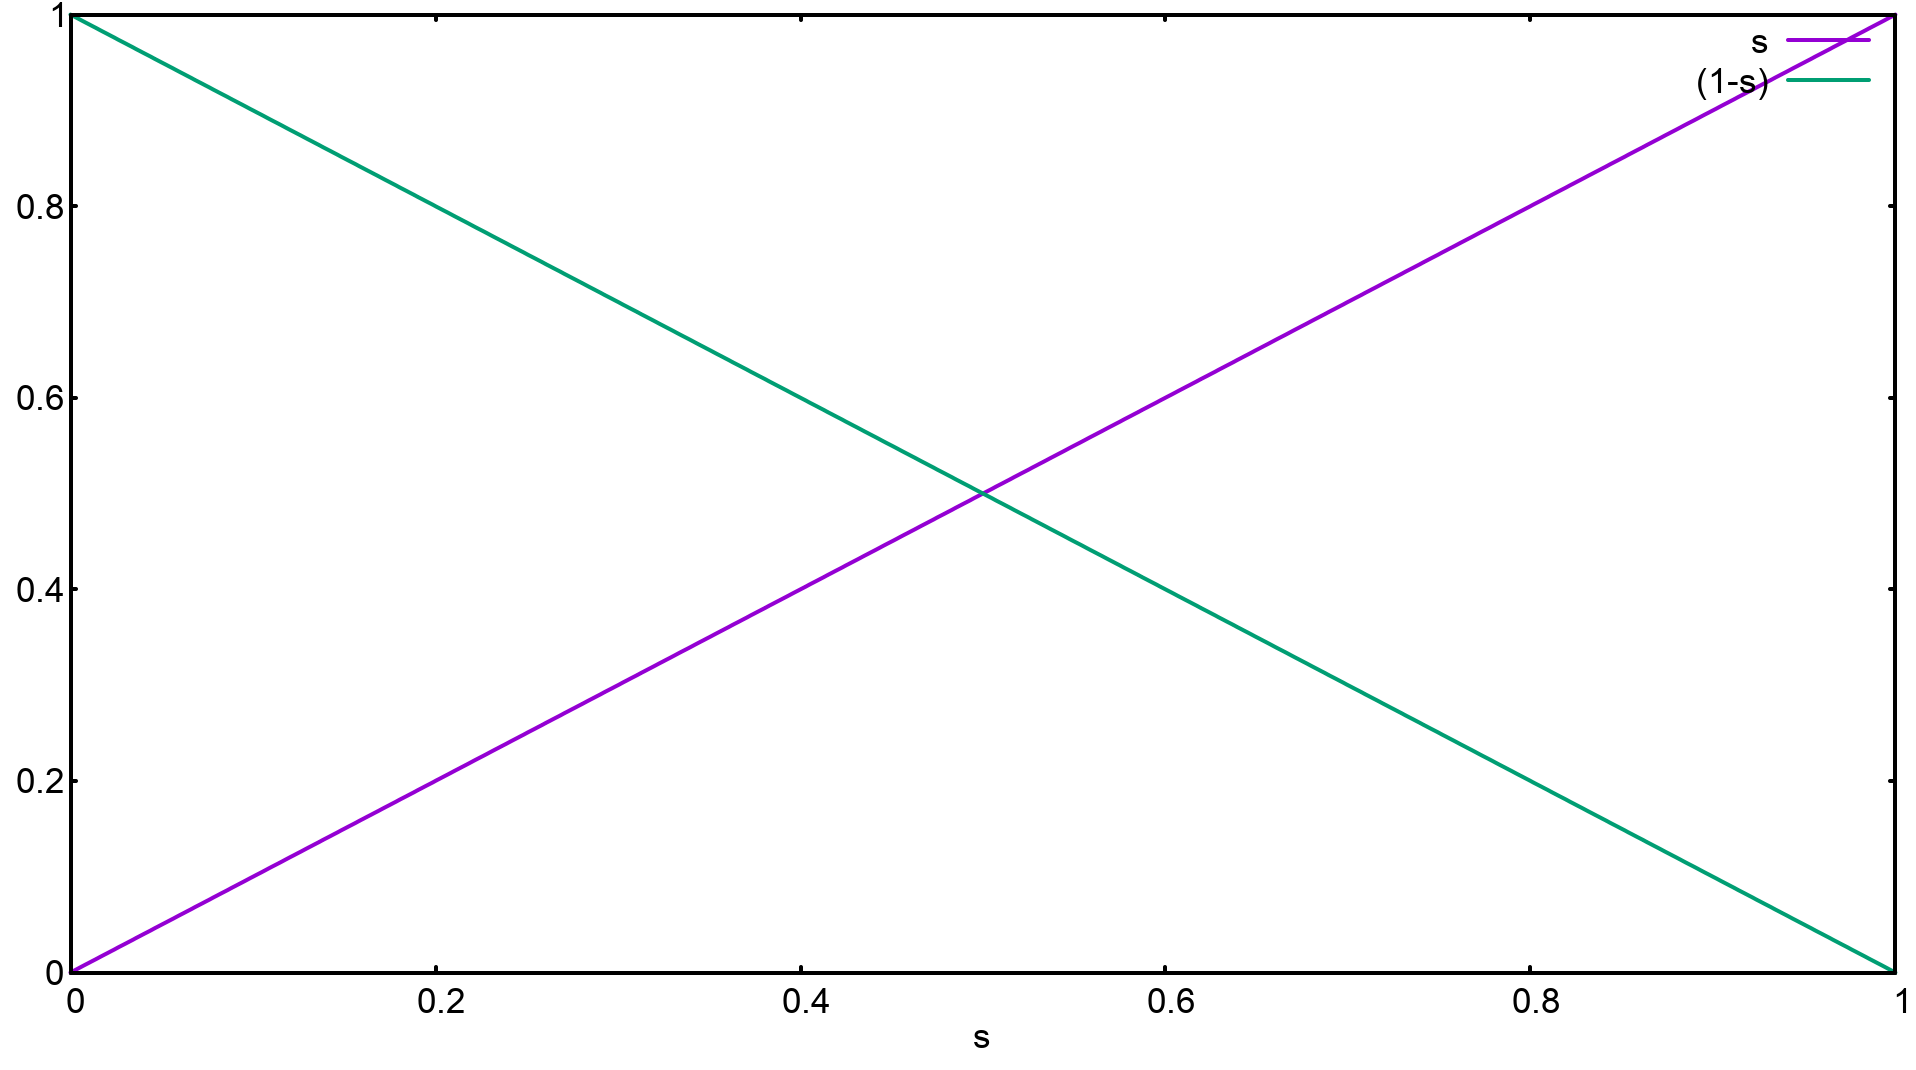
\includegraphics[scale=0.3]{Scheme.png}
\caption{The linear annealing scheme chosen, in terms of the annealing parameter s.}
\label{fig:b1}
\end{figure}
Therefore, the instantaneous Hamiltonian transitions from the initial Hamiltonian, $H(t=0)=H_I$ to the problem Hamiltonian, $H(t=T)=H_P$. \\

According to the \textbf{quantum adiabatic theorem}, the instantaneous state of the system stays close to the ground state of Hamiltonian H(t), if one starts with ground state of the initial Hamiltonian and if the driving from the initial Hamiltonian to the problem Hamiltonian is slow enough for the given minimum energy gap, $\Delta_{min}$, between the ground state and the first excited state of the Hamiltonian H(t) for t $\epsilon$ [0,T]. [ADIABATIC QUANTUM COMPUTATION, Enej Ilievsk]. Mathematically, adiabatic theorem of evolution holds when 
\begin{equation}
T>> {\Delta}_{min}^{-2}, \label{eq:b8}
\end{equation}
where T is the total annealing time. [Perspectives of quantum annealing: Methods and implementations].\\
Thus, the problem of finding the optimal solution reduces to the problem of solving the time dependent Schr{\"o}dinger equation for the resulting H(t) (equation \ref{eq:b7}):
\begin{equation}
i\frac{\partial}{\partial t}\ket{\psi}=H(t)\ket{\psi}.    \label{eq:b9}
\end{equation}

However, the process of evolution, starting from the trivial ground state of the initial Hamiltonian and going to a non-trivial ground state of the problem Hamiltonian, is accompanied by a quantum phase transition. For such a transition, the minimum gap $\Delta_{min}$ can be assumed to follow
\begin{equation}
\Delta_{min} \propto e^{-cN}, \label{eq:b10}
\end{equation}
for a positive constant c and N number of spins. [Perspectives of quantum annealing: Methods and implementations]. Substituting equation (\ref{eq:b10}) in equation (\ref{eq:b8}),
\begin{equation}
 T>> e^{2cN}, \label{eq:b11}
\end{equation}
i.e., the total annealing time required for the evolution to be adiabatic grows exponentially with the number of spins. This approach is therefore rendered unsuitable for systems with large number of spins.

However, altering the annealing scheme can help overcome this difficulty of an exponential increase in the computational resources with the number of variables [Perspectives of quantum annealing: Methods and implementations, Adiabatic quantum computation: Tameem Albash, Quantum Adiabatic Evolution Algorithms with Different Paths: Farhi, Different strategies for Optimization Using the Quantum Adiabatic Algorithm: Farhi, Nonstoquastic Hamiltonians and quantum annealing of an Ising spin glass]. In this work we include a third Hamiltonian, the Trigger Hamiltonian - $H_T$ in the time dependent Hamiltonian H(t) (equation \ref{eq:b7})[Farhi-Goldstein, Farhi (Different), Review, Non-stoquastic]. The trigger Hamiltonian is constituted by the transverse spin couplings $J_{ij}^x$. Moreover, $H_T$ should vanish at both the start and end of the annealing process, so that one can still start with the easily realizable ground state of the initial Hamiltonian, and the resulting state of the problem Hamiltonian remains unaffected. The instantaneous Hamiltonian thus takes the form: 
\begin{equation}
H(t)= (1-s)H_I + g*s(1-s)H_T + sH_P ,\label{eq:b12}
\end{equation} 
where parameter g controls the strength of the added trigger.\\
Furthermore, for this thesis we deal with two types of trigger Hamiltonians - The ferromagnetic trigger (F) and the anti-ferromagnetic trigger (A), given as
\begin{equation}
H_T^F = - \sum\limits_{<i,j>}{\sigma_i}^x{\sigma_j}^x,    \label{eq:b13}
\end{equation}
and
\begin{equation}
H_T^A= +\sum\limits_{<i,j>}{\sigma_i}^z{\sigma_j}^z,          \label{eq:b14}
\end{equation}
with the same pairwise coupling set $<i,j>$ as for the problem Hamiltonian.
\textbf{What else about these triggers? Frustration upon adding AF trigger, something about F too.)}
As will be seen in the following chapters, adding these triggers alter the energy spectrum considerably, which in turn affects the overlap of the final state with the ground state in different ways. \\


There can be yet another approach for increasing the overlap of the final state obtained from the annealing process, with the ground state of the problem Hamiltonian. As seen in (\ref{eq:b8}) for problems with small minimum gap $\Delta_{min}$, the annealing time required for the evolution to be adiabatic (so that the state of the system always stays close to the instantaneous ground state) can be very large. In such cases, even what otherwise looks like a reasonable time, might actually be short, causing the system to transit to the first excited state at the minimum gap anti-crossing. Since most of the amplitude of the state then lies in the first excited state, the overlap with the ground state might become negligible. 

However, if one chooses much smaller annealing times, the state can leak to higher excited states of the spectrum, even before the minimum gap anti-crossing. This gives the system a chance to shift some amplitude of the wave function back to the ground state at the minimum gap. Furthermore, the system can even end in a superposition state consisting of higher energy levels. As a result of this non-adiabatic evolution, the final state can have more chances of having a larger overlap with the ground state of the instantaneous Hamiltonian, than in the case of it closely following the first excited state with vanishing overlap with the ground state. This observation has been confirmed in the work by [Farhi et al: Different Perspectives], where reducing the total annealing time in problems with very small success probabilities, increases the probability of finding the final state close to the ground state of the problem Hamiltonian.\\

The following sections focus on two approaches that have been used in this work to solve the time-dependent Schr{\"o}dinger equation. Suzuki-Trotter product formula has been adopted to track the evolution of the state, and to compute the overlap of the final state with the already determined ground state of the problem Hamiltonian. The full diagonalization method, on the other hand, has been used to calculate the errors involved in using the Suzuki-Trotter approximation, and to determine the energy spectra and minimum gaps for H(t) for $t \in [0,T_A]$, where $T_A$ is the total annealing time.

\section{Exact Diagonalization}
This method consists of determining the eigenvalues and eigenvectors of the Hamiltonian matrix, which is a $L\times L$ ($2^N \times 2^N$) matrix, at each time step.

For constructing the Hamiltonian matrix at time step t $\in [0,T_A]$, all the basis vectors in the computational basis are acted upon by the instantaneous Hamiltonian, given by equation (\ref{eq:b12}). The action of the Hamiltonian on the $i^{th}$ basis vector corresponds to the $i^{th}$ column of the Hamiltonian matrix, e.g. for $\ket{\psi}=(1,0,...,0)^T$, $H\ket{\psi}$ gives the first column of the Hamiltonian matrix. \\
The resulting matrix is then diagonalized to obtain the eigenvalues $\Lambda$, and unitary matrix of the eigenvectors, V. Since $V^{\dagger}HV=\Lambda$, the unitary evolution operator $U(t)=e^{-itH}=Ve^{-it\Lambda}V^{\dagger}$.


This approach, however, has some serious limitations. Firstly, the memory requirement to store the Hamiltonian matrix grows exponentially with the number of qubits. Additionally, the full diagonalization takes $\mathcal{O}(2^{3N})$ floating-point operations [Kristel-Hans paper]. Therefore, this method is rendered impractical for solving the time dependent Schr{\"o}dinger equation for systems more than 20 qubits.

\section{Suzuki-Trotter Product Formula} 
Since solving the time dependent Schr{\"o}dinger equation requires to compute unitary matrix exponentials, Lie-Trotter-Suzuki product formula can be used to construct the following unitary approximations:
\begin{equation}
U(t)= e^{-itH}= e^{-it(H_1+...+H_K)}= \lim\limits_{m \to \infty} {\bigg(\prod_{k=1}^{K}e^{-itH_k/m} \bigg)}^m.    \label{eq:b15}
\end{equation}
For sufficiently small time step t, the first order approximation for U(t) in equation (\ref{eq:b15}) is
\begin{equation}
\tilde{U}_1(t)=e^{-itH_1}...e^{-itH_K},    \label{eq:b16}
\end{equation}
which holds good for $t \left| \left| H \right| \right| << 1$.

For an improved accuracy, a second order approximation is made to U(t) in equation (\ref{eq:b15}), using $\tilde{U}_1(t)$ from (\ref{eq:b16}):
\begin{equation}
\tilde{U}_2(t)=\tilde{U_1}^{\dagger}(-t/2)\tilde{U_1}(t/2)=e^{-itH_K/2}...e^{-itH_1/2}e^{-itH_1/2}...e^{-itH_K/2}.
\end{equation}
If $\tilde{U}_1(t)$ is unitary, so is $\tilde{U}_2(t)$. For unitary $\tilde{U}_2(t)$, the measure of error, calculated using the absolute difference between U(t) and $\tilde{U}_2(t)$ grows cubically in t [Kristel-Hans paper, 62 from there], i.e.
\begin{equation}
\left| \left| U(t)-\tilde{U}_2(t) \right| \right| \leq ct^3    
\end{equation} 
for a positive constant c. If the whole annealing process requires n such time steps, the involved error becomes
\begin{equation}
\left| \left| U(t)-\tilde{U}_2(t) \right| \right| \leq nct^3.  \label{eq:b17}
\end{equation}
Since $nt=T_A$, (\ref{eq:b17}) is equivalent to
\begin{equation}
\left| \left| U(t)-\tilde{U}_2(t) \right| \right| \leq cnT_At^2 = c't^2 \label{eq:b18}
\end{equation}
Substituting (\ref{eq:b5}),(\ref{eq:b13} or \ref{eq:b14}) and (\ref{eq:b4}) in (\ref{eq:b12}), we obtain:
\begin{equation}
H(t)=(1-s)\Big(-\sum \limits_{i=1}\limits^N h_i^x \sigma_i^x \Big)+g*s(1-s)\Big(\mp \sum \limits_{<i,j>}\sigma_{j}^x\Big) +s \Big(-\sum\limits_{i=1}\limits^{N}{h_i}^z{\sigma_i}^z - \sum\limits_{<i,j>}{J_{ij}^z} {\sigma_i}^z{\sigma_j}^z \Big).  \label{eq:b19}
\end{equation}
The Hamiltonian is then decomposed as follows:
\begin{equation}
H=H_{single}+H_x+H_z, \label{eq:b20}
\end{equation}
where $H_{single}=-(1-s)\Big(\sum \limits_{i=1}\limits^N h_i^x \sigma_i^x \Big)-s\Big(\sum\limits_{i=1}\limits^{N}{h_i}^z{\sigma_i}^z \Big)$, $H_x= \mp (1-s) \Big( \sum \limits_{<i,j>} J_{i,j}^x \sigma_{i}^x \sigma_{j}^x \Big)$, and $H_z= -s \Big(\sum \limits_{<i,j>} J_{i,j}^z \sigma_{i}^z\sigma_{j}^z\Big )$. In general, 
\begin{equation}
e^{i \mathbf{v.\sigma}}=cos(v) \mathbb{1} +i \frac{sin(v)}{v}\mathbf{v.\sigma},
\end{equation}
where $\mathbb{1}$ represents the identity matrix, and $v=\sqrt{v_x^2 +v_y^2 +v_Z^2}$. Then, 
\begin{equation}
e^{-itH_{single}}=\prod \limits_{i=1} \limits^{N} e^{it[(1-s)\sum \limits_i h_i^x \sigma_i^x +s \sum \limits_{i} h_i^z \sigma_i^z]} = \prod \limits_{i=1} \limits^{N} \begin{pmatrix}
cos(th_i) +i \frac{sh_i^z}{h_i} sin(th_i) &  i \frac{(1-s)h_i^x}{h_i} sin(th_i)\\
i \frac{(1-s)h_i^x}{h_i}sin(th_i) & cos(th_i) -i \frac{sh_i^z}{h_i} sin(th_i),
\end{pmatrix}
\end{equation}
where $h_i=\sqrt{(1-s(t))^2 {h_i^x}^2 + s(t)^2 {h_i^z}^2}$.\\

The computational basis states are the eigenstates of the Pauli-z operator, $\sigma_i^z$. Thus $e^{-itH^z}$ is a diagonal matrix in the computational basis, and its action on the input state changes the phase of each of the basis vectors. As $H^z$ is a sum of pair interactions, it is trivial to implement this operation as a sequence of multiplications by $4 \times 4$ diagonal matrices [Kristel-Hans paper].\\

The same approach can be adopted for implementing $H_x$ operations as well, by using the rotation operators $Y_j$ as follows. Writing $Y=\prod \limits_{i=1} \limits^{N} Y_i$, we obtain
\begin{equation}
e^{-itH^x}=\bar{Y}Y e^{-itH^z}\bar{Y}Y=\bar{Y}e^{it \sum \limits_{<i,j>} J_ij^x \sigma_i^z \sigma_j^z} Y.
\end{equation}

\end{document}